\begin{tikzpicture}
\node[inner sep=0,anchor=south west] (im) at (0,0) {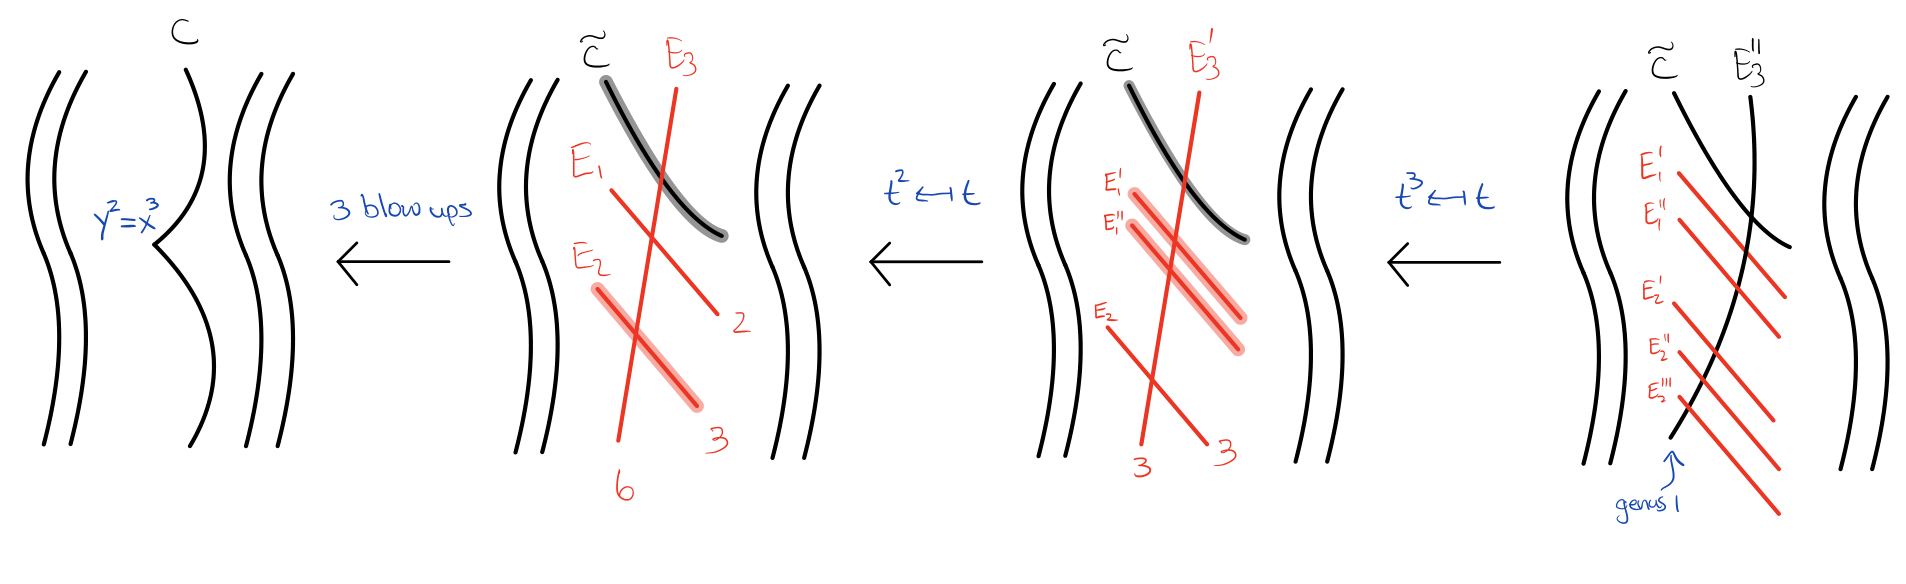
\includegraphics[width=.86\textwidth]{figures/reduction-cusp.png}};
\begin{scope}[x={(im.south east)},y={(im.north west)}]
\fill[white] (0.165,0.61) rectangle (0.26,0.75);
\fill[white] (0.46,0.62) rectangle (0.56,0.77);
\fill[white] (0.73,0.62) rectangle (0.81,0.77);
\fill[white] (0.845,0.09) rectangle (0.915,0.17);
\node[fill=white,inner sep=1pt,font=\scriptsize,text=blue] at (0.216,0.65) {$3$ 次爆破};
\node[fill=white,inner sep=1pt,font=\scriptsize,text=blue] at (0.5,0.675) {$t\mapsto t^2$};
\node[fill=white,inner sep=1pt,font=\scriptsize,text=blue] at (0.77,0.675) {$t\mapsto t^3$};
\node[fill=white,inner sep=1pt,font=\scriptsize,text=blue] at (0.88,0.13) {亏格 $1$};
\end{scope}\end{tikzpicture}
